%File: formatting-instructions-latex-2023.tex
%release 2023.0
\documentclass[letterpaper]{article} % DO NOT CHANGE THIS
\usepackage{aaai23}  % DO NOT CHANGE THIS
\usepackage{times}  % DO NOT CHANGE THIS
\usepackage{helvet}  % DO NOT CHANGE THIS
\usepackage{courier}  % DO NOT CHANGE THIS
\usepackage[hyphens]{url}  % DO NOT CHANGE THIS
\usepackage{graphicx} % DO NOT CHANGE THIS
\graphicspath{{images/}}

\urlstyle{rm} % DO NOT CHANGE THIS
\def\UrlFont{\rm}  % DO NOT CHANGE THIS
\usepackage{natbib}  % DO NOT CHANGE THIS AND DO NOT ADD ANY OPTIONS TO IT
\usepackage{caption} % DO NOT CHANGE THIS AND DO NOT ADD ANY OPTIONS TO IT
\frenchspacing  % DO NOT CHANGE THIS
\setlength{\pdfpagewidth}{8.5in}  % DO NOT CHANGE THIS
\setlength{\pdfpageheight}{11in}  % DO NOT CHANGE THIS
%
% These are recommended to typeset algorithms but not required. See the subsubsection on algorithms. Remove them if you don't have algorithms in your paper.
\usepackage{algorithm}
\usepackage{algorithmic}
\usepackage{bm}
\usepackage{amsmath}
%
% These are are recommended to typeset listings but not required. See the subsubsection on listing. Remove this block if you don't have listings in your paper.
\usepackage{newfloat}
\usepackage{listings}
\DeclareCaptionStyle{ruled}{labelfont=normalfont,labelsep=colon,strut=off} % DO NOT CHANGE THIS
\lstset{%
	basicstyle={\footnotesize\ttfamily},% footnotesize acceptable for monospace
	numbers=left,numberstyle=\footnotesize,xleftmargin=2em,% show line numbers, remove this entire line if you don't want the numbers.
	aboveskip=0pt,belowskip=0pt,%
	showstringspaces=false,tabsize=2,breaklines=true}
\floatstyle{ruled}
\newfloat{listing}{tb}{lst}{}
\floatname{listing}{Listing}
%
% Keep the \pdfinfo as shown here. There's no need
% for you to add the /Title and /Author tags.
\pdfinfo{
/TemplateVersion (2023.1)
}

\setcounter{secnumdepth}{0} %May be changed to 1 or 2 if section numbers are desired.

\title{Detecting Offensive Language in Tweets with Attention-fused Text and User Embeddings}
\author {
    % Authors
    Viha Gupta,\textsuperscript{\rm 1}
    Casey Primel\textsuperscript{\rm 1}
}
\affiliations {
    % Affiliations
    \textsuperscript{\rm 1} Dept. of Computer Science\\
    vg2237@nyu.edu, ctp219@nyu.edu
}



\begin{document}

\maketitle

\begin{abstract}
    Transformer-based models have come to dominate natural language processing tasks including semantic evaluation of social media content. Recent research demonstrates that the performance of such models can be improved by incorporating information about the online communities where that content is produced. For our project, we experiment with a novel method for incorporating community structure features  and text features to classify offensive language via attention mechanisms and positional encoding. In comparison to existing published solutions, we incorporate a "corrected" procedure for computing attention on graph-structured data to produce our user embeddings and a better performing pre-trained language model for our text embeddings. Our model achieves an F1 score of \textbf{FINAL SCORE} outperforming existing published results. Our code is available at \url{https://github.com/guptaviha/GF-OLD}.
\end{abstract}

\section{Introduction}

Content moderation is a pressing concern for online communities. For over a decade, automated systems have been employed to identify abusive behaviors and offensive language in user-generated content. Early systems relied on hand-crafted rules to extract linguistic features from textual data. Such rule-based systems have largely been replaced by neural network-based systems that can identify more subtle patterns in users' linguistic behaviors. However, research has shown that textual features are not always sufficient for identifying the nature of user-generated content. The rise of social media and the corollary ability to query the social graphs formed by users' activity has opened up a possible data source for constructing the requisite context. The remaining question is how to most effectively provide such context from the available data. Our project focuses on one solution in the context of Twitter: the fusion of text and user embeddings via attention mechanisms.

\section{Related work}

\subsection{Semantic evaluation of Twitter content}
Recent work exploring the application of deep learning for offensive language detection on Twitter can be divided into two different approaches. The first approach focuses solely on text data (e.g., tweets) and the use of pre-trained language models fine-tuned for this domain-specific task. \citep{liu2019-nuli}. DISCUSS TWEETEVAL


The second approach combines text data with information about users and community structure. Recent exemplars of this approach have used graph neural networks to learn the features of the social graph: \citet{Mishra2019} constructs a heterogeneous graph of users and tweets and applies a graph convolutional network to learn its features. \citet{Miao2022} begins by independently extracting text and user embeddings and then fusing them via attention mechanisms. The latter serves as the starting point for our project. EXPAND BOTH OF THESE.


\section{Methodology}

DESCRIBE OBJECTIVES.

\subsection{Dataset}

For this project, we will be using the English-language dataset collected, labeleled and made publicly available on GitHub by \citet{Miao2022}.\footnote{\url{https://github.com/mzx4936/GF-OLD-Dataset}} The data was obtained via the Twitter API\footnote{https://developer.twitter.com/en/docs/twitter-api} and contains data from 1,260 users and 12,780 of their tweets posted between Janauary 2018 and March 2021. The dataset also captures the social community in terms of the follower-network between these users with 8,877 such relationships.  

\subsection{Model architecture}

We will be following \citet{Miao2022} in using a graph attention network for learning user embeddings and attention mechanisms for fusing user features with tweet features; however, rather than using text embeddings from BERT, we will use the RoBERTa-based model pre-trained on tweets and fine-tuned for offensive language detection \citep{Barbieri2020}.\footnote{\url{https://huggingface.co/cardiffnlp/twitter-roberta-base-offensive}}

All the models discussed here use  focal loss function \citep{lin2017focal}, a modified cross entropy loss designed for dealing with class imbalance. It introduces a scaling factor $(1-p_t)^\gamma$ such that setting $\gamma > 0$ reduces the relative loss for easy examples and puts more emphasis on hard to classify examples. The function can be written

$$
FL(p_t) = \alpha \cdot (1 - p_t)^\gamma \log{p_t}
$$

where $p_t = \begin{cases} p, & \text{if } y =1 \\ 1-p, & \text{otherwise}  \end{cases}$, i.e., the magnitude of the estimated probabilty irrespective of the class label. In the special case where $\gamma=0$, the focal loss function simplifies to cross entropy loss.

\subsubsection{Transformer-based language models}

BERT AND DIFFERENCE BETWEEN BERT AND ROBERTA.

\subsubsection{Graph attention networks}

Graph attention networks (GAT) are an attention-based graph neural network (GNN) architecture for performing node classification of graph-structured data introduced by \citet{Vel2017}. Here, attention is used as a means of neighborhood aggregation wherein the hidden representation of each node in the graph is computed by attending over all its neighbors and selecting those which are most relevant.  Mathematically, GAT computes a score of every edge in the graph which indicates the importance of the features of a given node's neighbor to the given node, $e(\mathbf{h}_i, \mathbf{h}_j)=LeakyReLU(\bm{a}^T \cdot \lbrack \mathbf{Wh}_i || \mathbf{Wh}_j \rbrack)$, where both $\bm{a}$ and $\mathbf{W}$ are learned. From here, it computes a learned weighted average of the representations of a given node's neighbors followed by a nonlinearity. 

As noted by \citet{Brody2021}, the expressiveness of GAT as formulated by \citet{Vel2017} is constrained because the ranking of node importance computed as part of its scoring function ends up being shared by all nodes in the graph. \citet{Brody2021} refer to this as \textit{static attention} and demonstrate how static attention prevents GAT from approximating even very simple functions. To remedy this, \citet{Brody2021} suggest a simple reordering of the operations in GAT resulting in what they refer to as GATv2. The reordering separates out the application of $\bm{a}$ and $\mathbf{W}$ in the scoring function so that they do not collapse into a single linear layer: $e(\mathbf{h}_i, \mathbf{h}_j)=\bm{a}^T LeakyReLU(\mathbf{W} \lbrack \mathbf{h}_i || \mathbf{h}_j \rbrack)$. 

\citet{Miao2022} use GAT to derive their user embeddings prior to performing attention fusion. Because GAT exhibits static attention, the user embeddings derived emphasize global community structure and de-emphasize local structures within the social graph. We hypothesize that substituting GAT with GATv2 will allow the user embeddings to better express the local structures of the social graph.



\subsubsection{Attention fusion}

DESCRIBE HOW ATTENTION IS USED TO FUSE EMBEDDINGS.

\subsection{Training setup}

DESCRIBE TRAINING SETUP: SCRIPTS AND HARDWARE.

\subsection{Experiments}

DESCRIBE EXPERIMENTS RUN AND RATIONALE.

\section{Results}

\begin{figure*}
    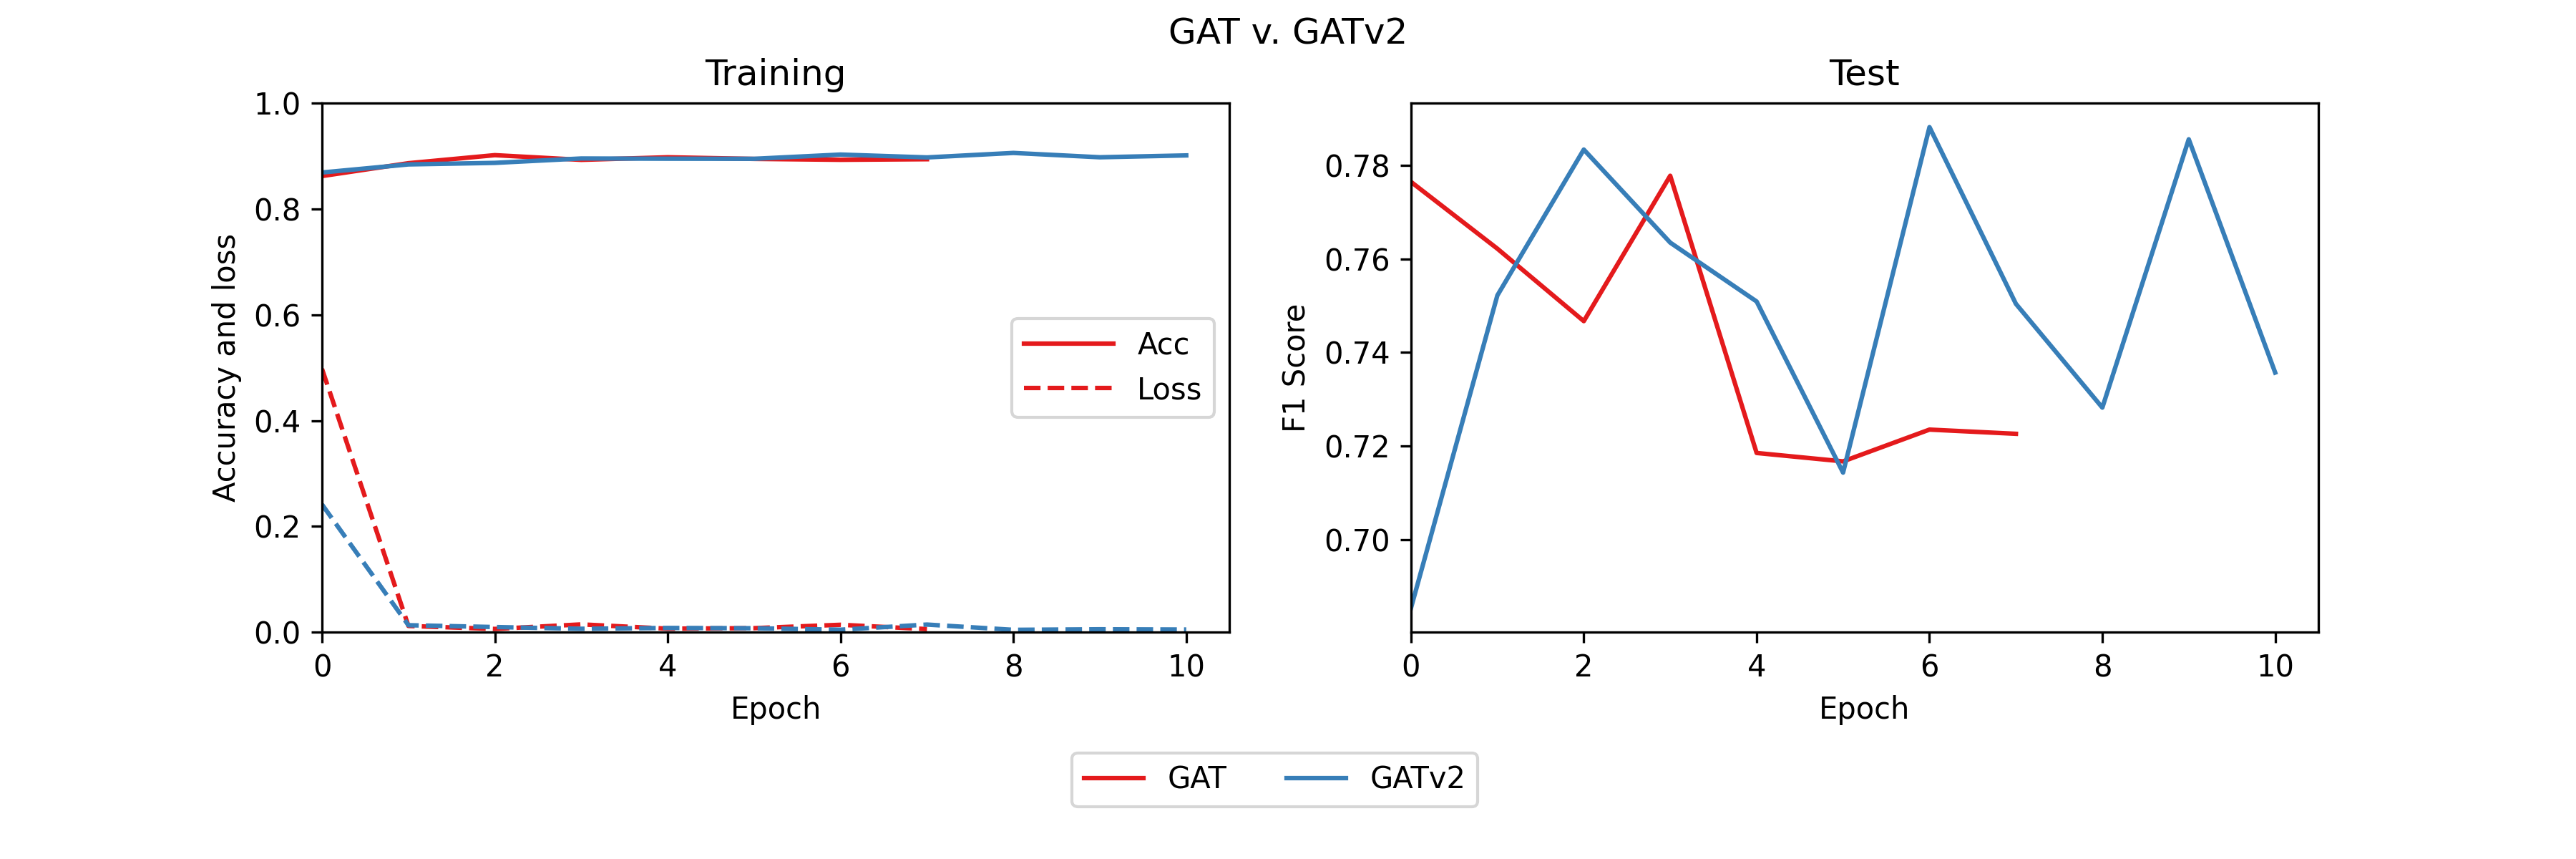
\includegraphics[width=\linewidth]{gat_v_gatv2.png}
    \caption{Comparison of model training accuracy, training loss and test F1 score for GAT and GATv2.}
\end{figure*}

\begin{figure*}
    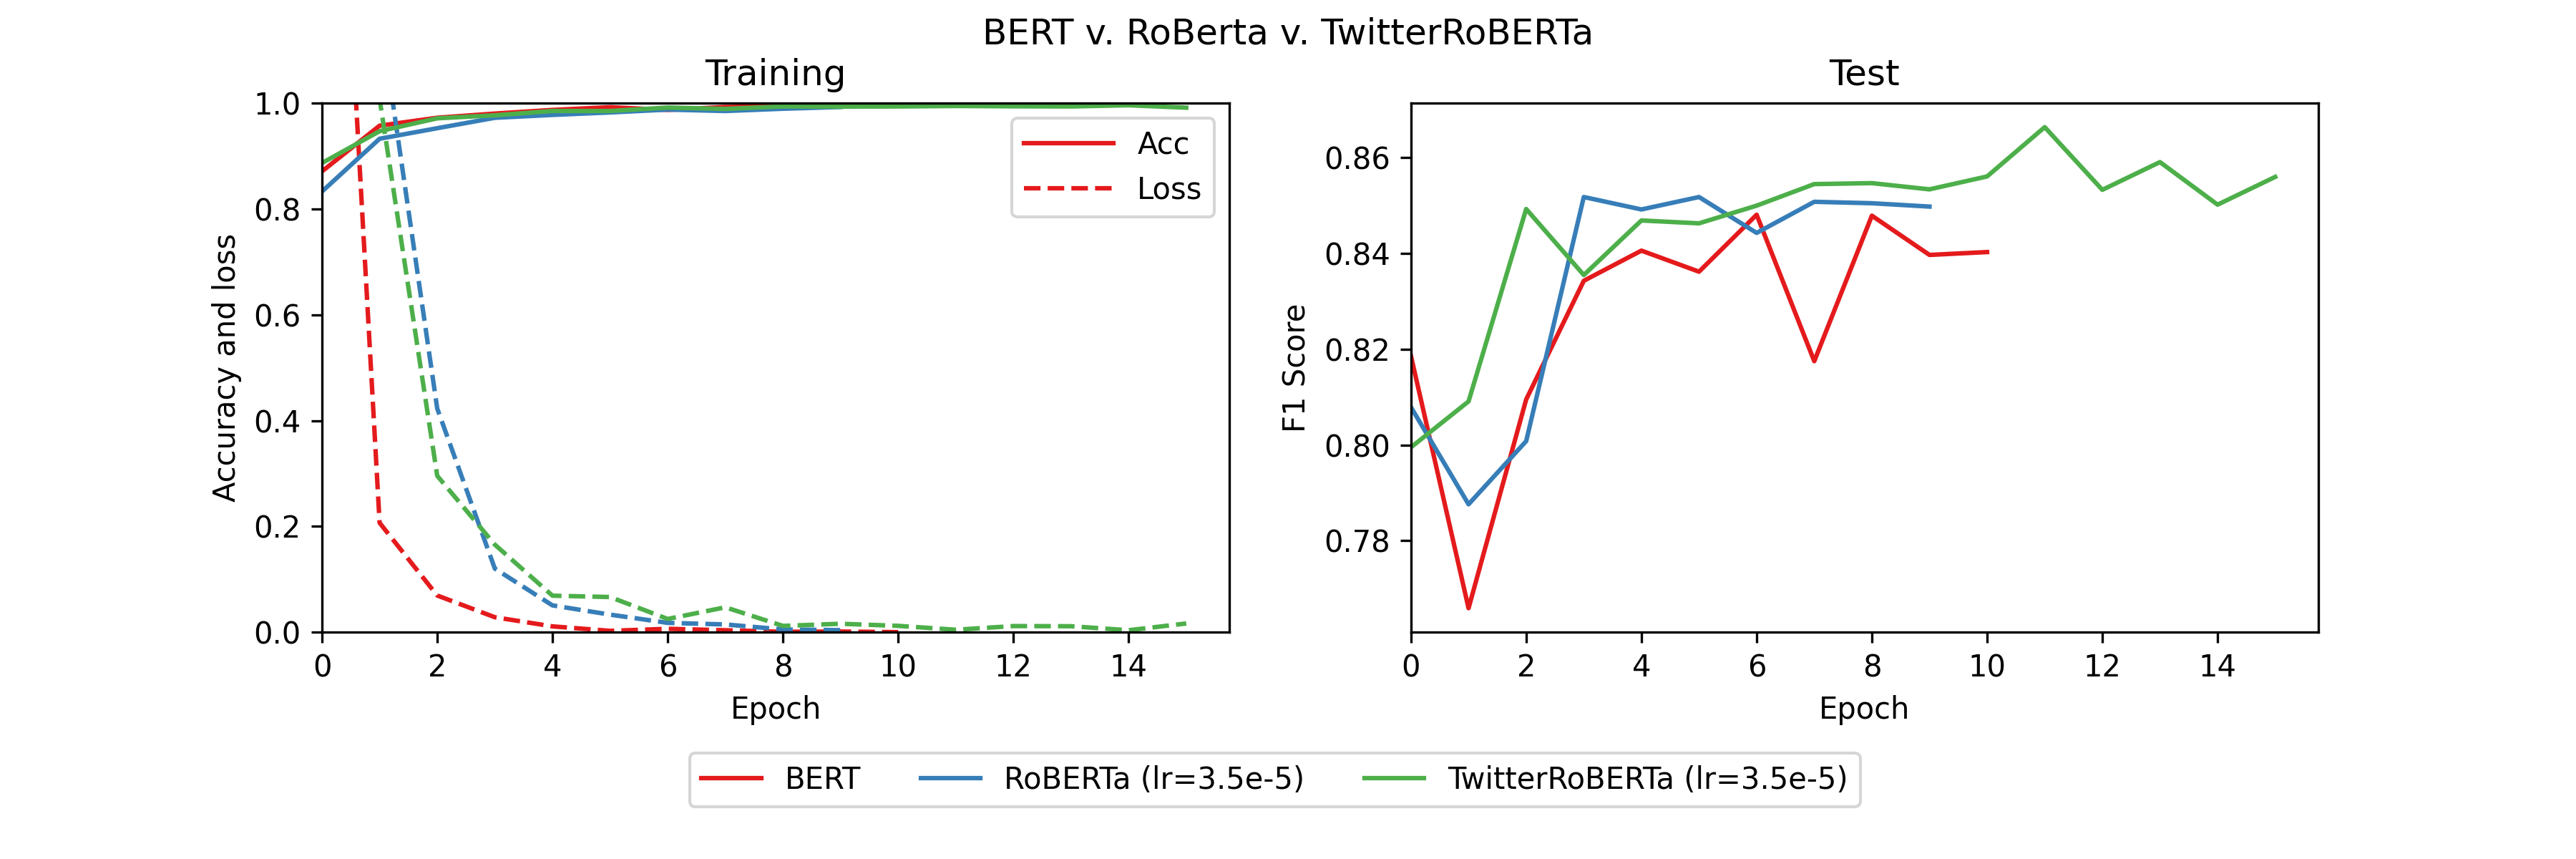
\includegraphics[width=\linewidth]{all_berts.png}
    \caption{Comparison of model training accuracy, training loss and test F1 score for BERT, RoBERTa and TwitterRoBERTa.}
\end{figure*}

\begin{figure*}
    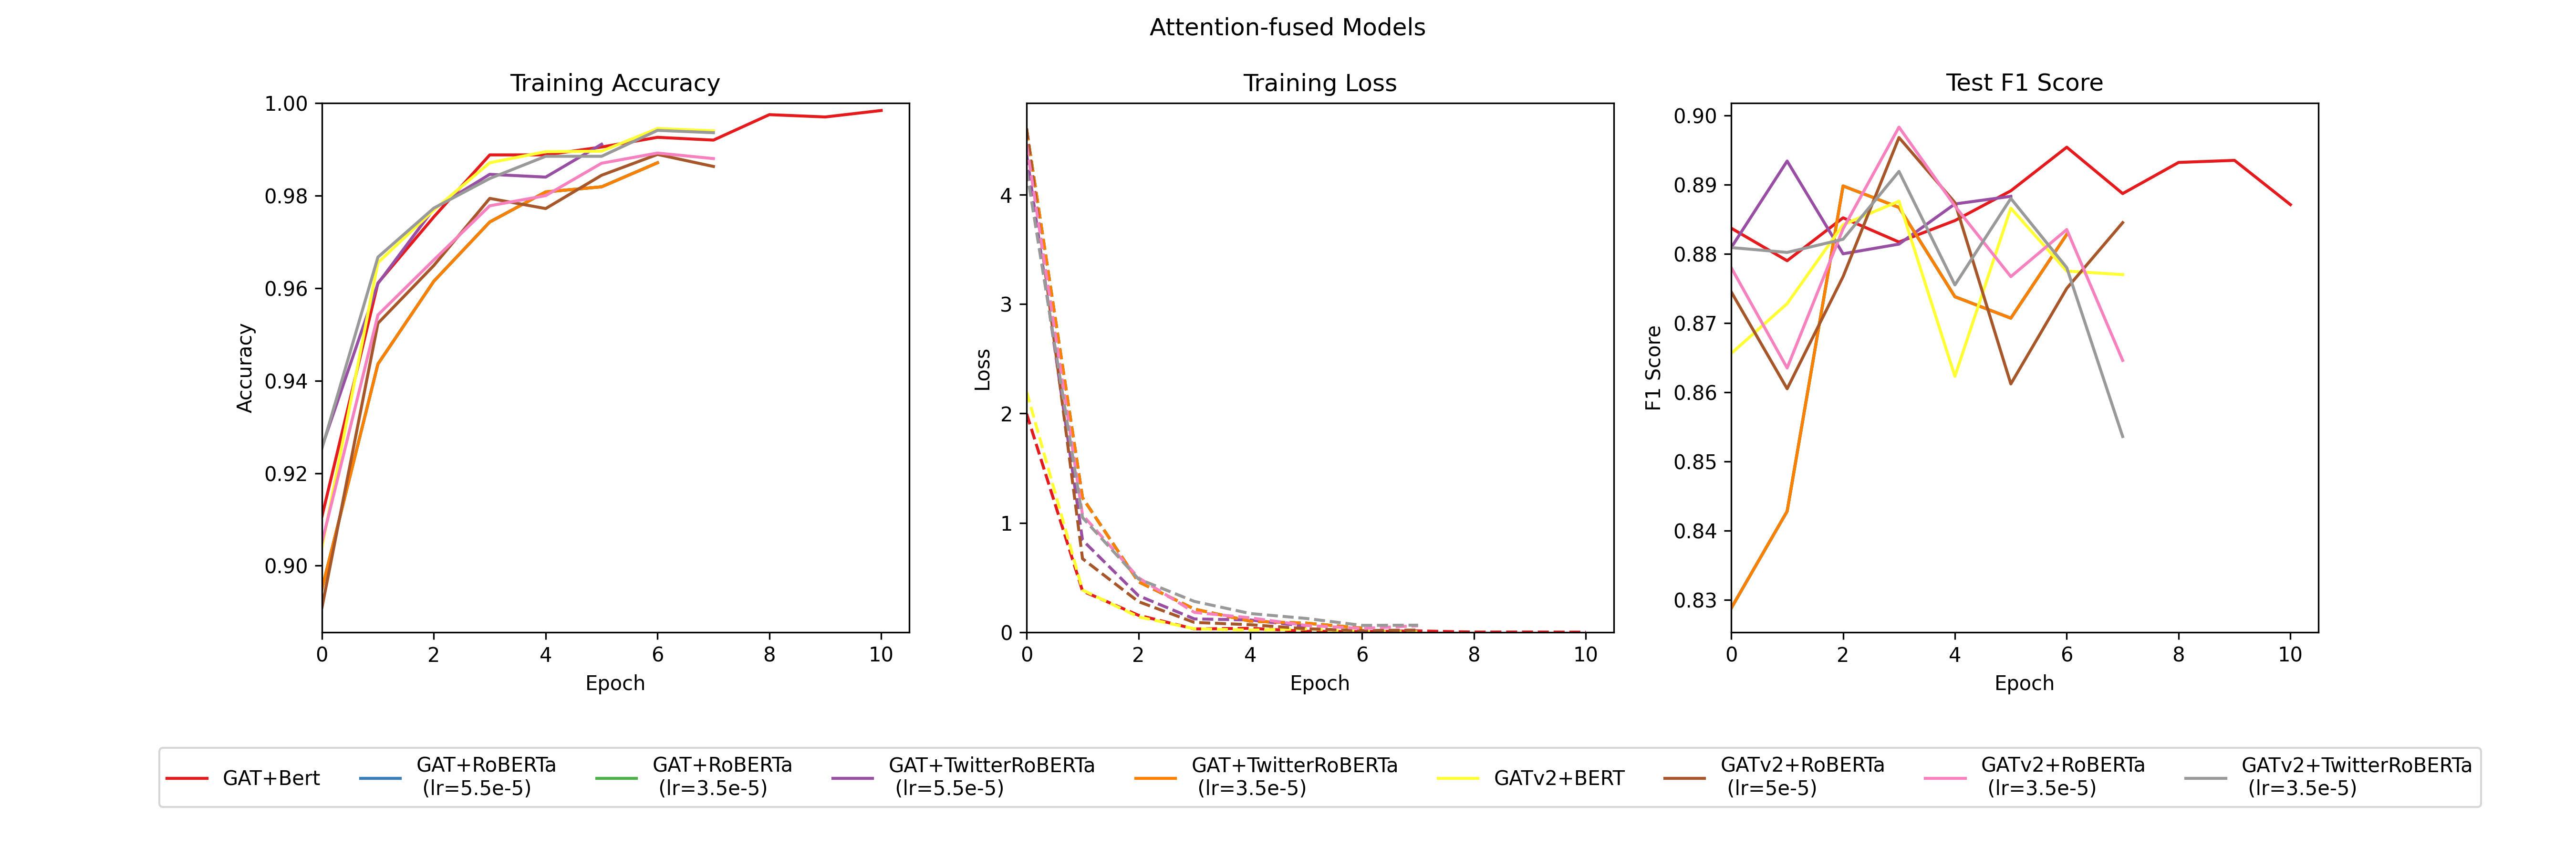
\includegraphics[width=\linewidth]{all_joint.png}
    \caption{Comparison of model training accuracy, training loss and test F1 score for all attention-fused models.}
\end{figure*}

SUMMARIZE RESULTS. SHOW LOSS + ACC PLOTS.

\section{Discussion}

More data + graph feature engineering. Hyperparameter tuning. Exploring different optimizers and LRs and regularization.

\appendix

\bibliography{project}

\end{document}